\capitulo{5}{Aspectos relevantes del desarrollo del proyecto}

%Este apartado pretende recoger los aspectos más interesantes del desarrollo del proyecto, comentados por los autores del mismo.
%Debe incluir desde la exposición del ciclo de vida utilizado, hasta los detalles de mayor relevancia de las fases de análisis, diseño e implementación.
%Se busca que no sea una mera operación de copiar y pegar diagramas y extractos del código fuente, sino que realmente se justifiquen los caminos de solución que se han tomado, especialmente aquellos que no sean triviales.
%Puede ser el lugar más adecuado para documentar los aspectos más interesantes del diseño y de la implementación, con un mayor hincapié en aspectos tales como el tipo de arquitectura elegido, los índices de las tablas de la base de datos, normalización y desnormalización, distribución en ficheros3, reglas de negocio dentro de las bases de datos (EDVHV GH GDWRV DFWLYDV), aspectos de desarrollo relacionados con el WWW...
%Este apartado, debe convertirse en el resumen de la experiencia práctica del proyecto, y por sí mismo justifica que la memoria se convierta en un documento útil, fuente de referencia para los autores, los tutores y futuros alumnos.

%Despliegue continuo - direccion de app en heroku. Sistema gratuito sirve para validar, pero no para explotar
%Diseño extensible
%Framework vaadin
%No responsive

En este capítulo se recogen los aspectos más interesantes del desarrollo del proyecto y se justifican las diferentes decisiones tomadas durante el mismo. Se hace mención al motivo de elección del proyecto, el modelo del ciclo de vida empleado, el flujo de trabajo y la configuración del proyecto.


\section{Selección del proyecto}

La elección de este proyecto se debe a su temática de análisis de repositorios. Trata un aspecto al que normalmente no se presta demasiada atención en el desarrollo de proyectos software. Según la experiencia laboral del alumno, normalmente se presta más atención a métricas de proyecto y se descuidan las del proceso, olvidando cuidar la administración de la calidad correctamente.
Esto es un error ya que analizando los repositorios con los que trabajamos en el desarrollo de proyectos podemos obtener métricas que nos dan información muy valiosa. Con esta información podemos detectar problemas que antes pasaban desapercibidos y mejorar en mucho la productividad de los equipos modificando ciertos aspectos del proceso de desarrollo.
En este proyecto se han utilizado métricas que permiten llevar un control sobre el ciclo de vida de uno o varios proyecto, haciendo posible comparar su evolución a lo largo del tiempo. Además, permiten comparar si se están cumpliendo los objetivos definidos y como se mencionaba anteriormente mejorar el proceso de desarrollo aumentando su calidad.

En cuanto a la relación del proyecto con las diferentes asignaturas del Grado, está principalmente relacionado con la asignatura \textit{Desarrollo Avanzado de Sistemas Software}, donde se trata como desarrollar software de calidad mediante el proceso de \textit{Administración de la calidad}, en el cual una de las actividades es el control de calidad. Este control se puede llevar a cabo mediante un proceso de medición utilizando diferentes métricas.


Otras asignaturas relacionadas: 
\begin{itemize}
	\tightlist
	\item \textit{Metodología de la Programación} y \textit{Estructuras de Datos} han contribuido en cuanto a la construcción de una aplicación en un lenguaje Orientado a Objetos.	
		\item \textit{Ingeniería del Software}: ciclo de vida del software, el análisis de los requisitos y el modelado del sistema (diagramas de clases, diagramas de casos de uso, etc).
		\item \textit{Análisis y Diseño de Sistemas}: comprensión del sistema desarrollado en la aplicación Web ya existente \cite{TFGPrevio} de forma que se puedan realizar nuevas implementaciones y mejoras.
	\item \textit{Estadística}: comprensión del cálculo de cuartiles para calcular los valores umbrales de las métricas.
	\item \textit{Interacción Hombre/Máquina}: comprensión de los aspectos fundamentales para mejorar la usabilidad, simplicidad, adaptabilidad de la interfaz gráfica.
	\item \textit{Diseño y Mantenimiento del Software}, el uso de patrones de diseño para mejorar la calidad de código y mantener los principios SOLID  \footnote{Single responsability, Open/Closed, Liskov substitution, Interface segregation, Dependency inversion} y de \textit{Desarrollo Avanzado de Sistemas Software} la naturaleza del trabajo, las revisiones automáticas de calidad de código por medio de métricas y la importancia de la refactorización al detectar defectos de diseño.
	\item \textit{Validación y Pruebas} comprensión de las pruebas ya desarrolladas y construcción de nuevas.
	\item \textit{Sistemas Distribuidos} ha ayudado en el uso de Maven y en la construcción de una aplicación Web.
	\item \textit{Gestión de Proyectos}: ciclo de vida de desarrollo empleado durante el proyecto: \textit{Scrum}\cite{scrum_master_scrum_2019}.
\end{itemize}

\newpage

\section{Modelo de ciclo de vida}
La metodología utilizada durante el desarrollo del proyecto ha sido \textit{\textbf{Scrum}}, realizándose un proceso incremental, dividido en \textit{sprints} de dos semanas. A la finalización de cada \textit{sprint} se ha realizado una reunión denominada \textit{sprint review} que que se compone de dos partes:
\begin{description}
	\item [Revisión del sprint:] o \textit{sprint review}, donde se comentan los avances realizados así como los diferentes problemas que han surgido durante las dos semanas de duración del \textit{sprint}.
Se modifica la pila de desarrollo (\textit{sprint backlog}) pasando a completadas aquellas historias de usuario finalizadas y al siguiente \textit{sprint} las no finalizadas, comentando posibles mejoras y soluciones a los problemas que se hayan tenido \cite{scrum_master_scrum_2019}.

	\item [Planificación del siguiente sprint:] o \textit{sprint planning}, donde e definen las tareasa abordar  durante el siguiente sprint. Estas tareas se recogen del \textit{product backlog} o pila de producto y se añaden a la pila del sprint o \textit{sprint backlog}.
\end{description}

	Concretamente, se ha utilizado \textbf{ZenHub} en conjunto a las \textit{issues} de GitHub para la gestión del proceso \textit{Scrum} en el proyecto.

A lo largo del desarrollo del proyecto, los \textit{sprints} se han centrado en diferentes tareas como pueden ser:
\begin{itemize}
	\item  Tareas de \textbf{investigación}, tanto de las materias relacionadas con el proyecto como de las herramientas que se utilizarán durante el proceso y de \textbf{configuración} del entorno de desarrollo.
	\item En la segunda etapa se aprecian tareas de \textbf{diseño e implementación} de la parte lógica de la aplicación. Se diseña el framework de conexión a forjas de repositorios, se implementa el framework descrito en \textit{Soporte de Métricas con Independencia del Lenguaje para la Inferencia de Refactorizaciones}  \cite{marticorena_sanchez_soporte_2005} para el cálculo de métricas y se diseñan los modelos de datos que serán utilizados por la aplicación.
	\item Tareas de \textbf{desarrollo} de las nuevas funcionalidades del proyecto, como la integración con GitHub, utilizando como base el framework descrito en \textit{Soporte de Métricas con Independencia del Lenguaje para la Inferencia de Refactorizaciones}  \cite{marticorena_sanchez_soporte_2005} y la integración ya existente con GitLab. Nuevos tests y mejoras de diferentes interfaces.
	\item Tareas de \textbf{integración y despliegue continuo} (CI/CD), configurando GitHub Actions y el resto de herramientas para el flujo de trabajo de los sprints.
	\item Revisión de las \textbf{pruebas unitarias} existentes y creación de nuevas con JUnit. automatizando su ejecución gracias a Maven y los \textit{pipelines} \footnote{Definen las actividades de los procesos de CI/CD y las fases y el entorno en las que se ejecutarán} de GitHub Actions.
		\item Configurar \textbf{revisiones automáticas de calidad} y de cobertura de las pruebas gracias a Maven, Codacy, JaCoCo y GitHub.
	\item Configuración y puesta a punto de un entorno en Heroku donde realizar el \textbf{despliegue} la aplicación durante las tareas de de CI/CD.
	\item Revisión y configuración de \textbf{badges} \footnote{Distintivos que aportan información rápida sobre el estado del proyecto en ciertos aspectos como la cobertura, la calidad de código o el proceso de CI/CD y enlazan con la fuente de información} para representar el estado del proyecto en cuanto a calidad de código, cobertura, despliegue y los trabajos de CI/CD.
	\item Implementación de mejoras y nuevos aspectos relacionados con la nueva funcionalidad en la \textbf{interfaz gráfica}.
	\item Tareas de \textbf{documentación} en la que se trabaja sobre la memoria y los anexos.
\end{itemize}

Consultando el \textit{Anexo A - Plan de Proyecto Software} se puede obtener más información sobre los \textit{sprints} realizados y el ciclo de vida del proyecto.

\section{Gestión del proyecto}

En esta sección se explican los diferentes aspectos relacionados con la gestión y configuración del proyecto.

\subsection{Aplicación Web}

Se trabaja sobre la aplicación web implementada en la primera iteración del proyecto\cite{TFGPrevio}.
Un aplicación web tiene como ventajas: 
\begin{itemize}
	\tightlist
	\item El usuario puede acceder a ella directamente desde el navegador, sin necesidad de realizar instalación.
	\item  Al no necesitar instalación, se puede utilizar desde cualquier dispositivo que tenga instalado algún navegador Web. Se ha comprobado la compatibilidad de la aplicación con los siguientes: \textit{Mozilla Firefox}, \textit{Microsoft Edge}, \textit{Internet Explorer}, \textit{Google Chrome} y \textit{Opera}.
	\item Actualizaciones. Para actualizar una aplicación Web, el usuario final no tiene que instalar la actualización. Sino que habrá un periodo de mantenimiento de aplicación, normalmente muy corto y fuera de horario de uso, en el que ningún usuario podrá acceder a la aplicación. Después de este periodo, todos los usuarios dispondrán de la actualización.
	\item En cuanto a la actualización de la aplìcación web, los usuarios finales obtendrán la nueva versión en cuanto vuelvan a a acceder a la misma. Para evitar problemas de cacheo en el navegador se suele trabajar con \textit{Service Workers} que permiten la actualización de la web incluso cuando el usuario la está usando.
\end{itemize}


\subsection{Logo de la aplicación}

\begin{figure}[!h]
	\centering
	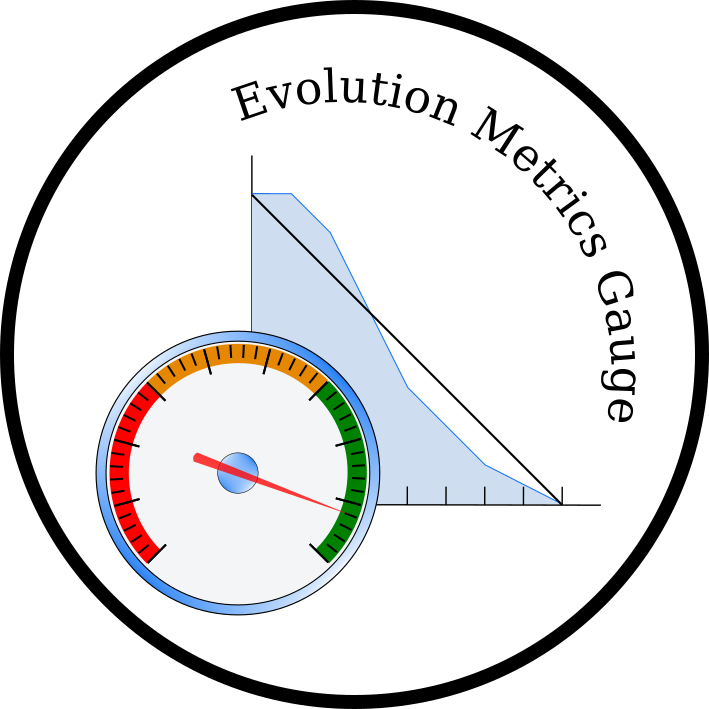
\includegraphics[width=0.5\textwidth]{_LOGOAPP}
	\caption{Logo de Evolution Metrics Gauge}\label{fig:_LOGOAPP}
\end{figure}
\FloatBarrier

En la Fig. \ref{fig:_LOGOAPP} se muestra el logo de la aplicación que se ha mantenido al tratarse este proyecto de una nueva iteración. Éste se compone de un tacómetro que simboliza la medición y un gráfico \textit{burndown} que simboliza la evolución de un proyecto. Lo que se pretende es mostrar la funcionalidad principal de la aplicación: calcular métricas de evolución.


\subsection{Java 11}
% TODO-> actualizar a Java17 si finalmente actualizamos el proyecto
Se ha mantenido la versión utilizada en el proyecto original\cite{TFGPrevio}, Java 11.
Para esta versión, la configuración necesaria de Maven para que el proyecto compile es la siguiente \ruta{pom.xml}:

%Tomcat \footnote{Para desplegar aplicaciones con Java 11 se requiere de la versión 9.0.x de Tomcat} y 
% del proyecto para que Maven compile en la versión 11 de Java:

\begin{minipage}{\linewidth}
{\tiny
\begin{verbatim}[breaklines]
...
<properties>
	<project.build.sourceEncoding>UTF-8</project.build.sourceEncoding>
	<project.reporting.outputEncoding>UTF-8</project.reporting.outputEncoding>
	<java.version>11</java.version>
</properties>
...
<build>
...
	<plugins>
		<plugin>
			<groupId>org.apache.maven.plugins</groupId>
			<artifactId>maven-compiler-plugin</artifactId>
			<configuration>
				<source>${java.version}</source>
				<target>${java.version}</target>
			</configuration>
			<version>3.8.0</version>
		</plugin>
		<plugin>
			<groupId>org.apache.maven.plugins</groupId>
			<artifactId>maven-war-plugin</artifactId>
			<version>3.2.2</version>
		</plugin>
		...
	</plugins>
	...
</build>
...
\end{verbatim}
}
\end{minipage}

Y en Eclipse IDE habría que añadir manualmente el JRE desde la ventana Window/Preferences, como se muestra en la siguiente figura: %Fig. \ref{fig:M5_Eclipse_Java11}.

%TODO imagen con la versión de Java que finalmente adoptemos

% \imagen{M5_Eclipse_Java11}{Añadir Java 11 a Eclipse}

% TODO pendiente de adaptar con la version final de Java adoptada
%De la utilización de Java 11 destacan dos aspectos ya existentes en el proyecto:          
%	\item De la versión 11 se ha utilizado el método \textit{isBlank()} de la clase \textit{String} \footnote{\url{https://docs.oracle.com/en/java/javase/11/docs/api/java.base/java/lang/String.html}}. Se diferencia de \textit{isEmpty()} en que no comprueba la longitud de la cadena y devuelve \textit{true} si es 0. Sino que devuelve \textit{true} si la longitud es 0, o si no es 0 pero todos los caracteres de la cadena son espacios en blanco.
%	\item De la clase \textit{java.util.Optional} \footnote{\url{https://docs.oracle.com/en/java/javase/11/docs/api/java.base/java/util/Optional.html}}, soportada desde la versión 1.8, se utiliza la función \textit{orElseThrow()}, que se soporta desde la versión 10, por tanto habría que buscar una alternativa para pasar a la versión 1.8. La versión 11 trae a esta clase la función \textit{isEmpty()}.
%\end{itemize}
%
%Para saber más sobre las novedades de Java 11 es recomendable leer `\textit{JDK 11 Release Notes}' \cite{oracle_jdk_nodate}. También hay un artículo que explica las principales diferencias entre Java 8 y Java 11 llamado `\textit{De Java 8 a Java 11, ¿aún no te has migrado?}' \cite{del_hoyo_java_2019}.

\subsubsection{Trabajo con streams de Java}

Los \textit{Streams}, presentes en Java desde la versión Java 1.8 son muy útiles ya que facilitan enormemente el procesamiento de grandes colecciones de datos. Estos permiten, usando un predicado, \textbf{filtrar} datos de una colección, \textbf{ordenar} los datos mediante un comparador, \textbf{mapear} o \textbf{reducir} los datos mediante alguna función y \textbf{almacenarlos} en algún tipo de colección mediante un colector. \\ 
Destacan dos funcionalidades, el \textit{mapeo} que asocia cada dato del stream con un nuevo elemento (como el cálculo del cuadrado de cada elemento) y la \textit{reducción} que permite obtener un único resultado a partir del conjunto de datos (como la suma de un conjunto de datos).

Un ejemplo de uso de \textit{streams} en la aplicación:\\
\begin{minipage}{\linewidth}
{\tiny
\begin{verbatim}[breaklines]
...
return gitLabApi.getIssuesApi().getIssuesStream(projectId, new IssueFilter().withState(IssueState.CLOSED))
  .filter(issue -> issue.getCreatedAt() != null && issue.getClosedAt() != null)
  .map(issue -> (int) ((issue.getClosedAt().getTime() - issue.getCreatedAt().getTime()) / (1000 * 60 * 60 * 24 )))
  .collect(Collectors.toList());
...
\end{verbatim}
}
\end{minipage}

En el ejemplo se obtiene de GitLab API un \textit{stream} con las issues cerradas de un proyecto. Este \textit{stream} es filtrado y se obtienen aquellas que tengan fecha de creación y fecha de cierre (\textit{filter}), se calcula de cada \textit{issue} la diferencia en días entre la fecha de creación y la fecha de cierre (\textit{map}), y se recogen los resultados en una lista (\textit{collect}).

%TODO poner otro ejemplo cuando tengamos un acceso a la API de GitHub funcionando

\subsubsection{Interfaces funcionales y funciones lambda de Java}

EN el proyecto también se hace uso de interfaces funcionales y funciones lambda. En la sección anterior ya vemos el uso de dos funciones lambda en el código mostrado (argumentos de las funciones \textit{filter} y \textit{map}).

El paquete \textit{java.util.function} \footnote{\url{https://docs.oracle.com/javase/8/docs/api/java/util/function/package-summary.html}} es soportado por Java desde la versión 1.8. Este paquete permite almacenar funciones en variables. 
\\Las funciones lambda son funciones anónimas con sintaxis \\
\begin{minipage}{\linewidth}
{\tiny
\begin{verbatim}
(parametros) -> {cuerpo funcion lambda}
\end{verbatim}
}
\end{minipage}
que no están declaradas en una clase y pueden ser utilizadas en cualquier parte, pasarse como parámetro a una función y ser almacenadas en variables.
\\Las interfaces funcionales \footnote{\url{https://docs.oracle.com/javase/8/docs/api/java/lang/FunctionalInterface.html}} son interfaces con un único método, que es abstracto, llamado método funcional. Este método permite restringir los tipos de los parámetros y de los valores de retorno de una función lambda.

Estas han sido utilizadas en numerosas ocasiones tanto para los \textit{streams} (como se observa en el código anterior), como en elementos de la interfaz gráfica y otros elementos sensibles a eventos:\\
\begin{minipage}{\linewidth}
{\tiny
\begin{verbatim}[breaklines]
...
closeConnectionButton.addClickListener(event ->  
{
  if(rds.getConnectionType() != EnumConnectionType.NOT_CONNECTED) {
	try {
	  rds.disconnect();
	} catch (RepositoryDataSourceException e) {
		...
	}
  }
  close();
  connectionFormDialog.open();
});
...
\end{verbatim}
}
\end{minipage}

También han sido utilizadas para almacenar funciones en variables, definiendo una interfaz funcional para restringir los tipos parámetros y de los resultados de la función. Un aspecto importante es que las variables que almacenen funciones NO se pueden serializar, por eso la variable \textit{EVAL\_FUNC\_GREATER\_THAN\_Q1} del código siguiente se ha marcado como \textit{transient} dentro de una clase que implementa \textit{Serializable}.

\begin{minipage}{\linewidth}
{\tiny
\begin{verbatim}[breaklines]
...
public interface Metric extends Serializable {
 @FunctionalInterface
 public interface EvaluationFunction {
   EvaluationResult evaluate(IValue value, IValue minValue, IValue maxValue);
 }

 ...
 
 EvaluationResult evaluate(IValue measuredValue);

 EvaluationFunction getEvaluationFunction();
}

...
public abstract class NumericValueMetricTemplate implements Metric {
  ...
  protected transient static final EvaluationFunction EVAL_FUNC_GREATER_THAN_Q1 = 
    (measuredValue, minValue, maxValue) -> 
     {
      try {
        Double value, min;
	    value = ...
	    min = ...
	    if (value > min) return EvaluationResult.GOOD;
	    else if (value.equals(min)) return EvaluationResult.WARNING;
	    else return EvaluationResult.BAD;
	  } catch (Exception e){
	    return EvaluationResult.BAD;
	  }
    };
  ...
}
...
\end{verbatim}
}
\end{minipage}

En el ejemplo anterior muestra la manera en la que las métricas podrían valorarse. La métrica será dada como buena si supera el umbral inferior. Cada métrica podrá usar esta función o implementar una función propia si es necesaria una mayor particularización. Los requisitos definidos en la interfaz funcional son que esa función deberá tener tres argumentos del tipo \textit{IValue} y devolver un resultado del tipo \textit{EvaluationResult}.

\subsection{Maven}

Maven es una herramienta de gestión de proyectos software. Esta herramienta facilita, a partir de un único fichero con extensión \textit{XML} llamado \ruta{pom.xml} \footnote{Project Object Model}:
\begin{itemize}
	\tightlist
	\item La construcción y compilación del proyecto.
	\item La generación de documentación.
	\item La generación de informes.
	\item La gestión de las dependencias del proyecto.
	\item La integración con un sistema de control de versiones como Git, y el trabajo con repositorios remotos como GitLab o GitHub e incluso en repositorios \textit{self-hosted} \footnote{Repositorios almacenados en servidores gestionados por la propia empresa o equipo que desarrolla el software}.
	\item La generación y distribución de \textit{releases}.
\end{itemize}
Maven puede crear la estructura de directorios del proyecto, administrar las dependencias y descargar las librerías necesarias. Además, es compatible con la mayoría de IDEs \footnote{Integrated Development Environment - Entorno de desarrollo integrado}. Por ejemplo, en este proyecto se ha trabajado sobre Eclipse IDE, el cual tiene muy buena integración con Maven, como se puede observar en la Fig. \ref{fig:M5_Eclipse_Maven}.

\imagen{M5_Eclipse_Maven}{Integración de Maven con Eclipse}

También permite el uso de arquetipos, que son patrones o plantillas que se aplican en la infraestructura del proyecto.

Aunque puede resultar difícil configurar correctamente Maven a través del archivo de configuración, debido sobre todo al buen número de herramientas a configurar en él, una vez configurado, nos ahorra mucho tiempo y nos permite centrarnos en el desarrollo de funcionalidad.

\subsection{Sistema de control de versiones}

Se ha utilizado Git para el desarrollo del proyecto para el control de versiones y se ha utilizado GitHub como repositorio remoto. 

GitHub no sólo ha permitido el almacenamiento del código del proyecto si no que también ha permitido el seguimiento y colaboración alumno-tutor gracias a las herramientas que proporciona. Además, utilizando ZenHub (que se puede integrar en el propio GitHub) se ha llevado a cabo la gestión de las tareas (\textit{issues}) del proyecto. Como se puede observar en la Fig. \ref{fig:M5_GitHub-ZenHub_board}.

\imagen{M5_GitHub-ZenHub_board}{Tablero de Scrum en ZenHub integrado en GitHub}

Es posible configurar Eclipse y Maven para trabajar con Git. Sin embargo, debido a la costumbre de uso directamente en consola del alumno, se ha optado por el uso de GitBash tal y como se muestra en la Fig. \ref{fig:M5_GitBash}.

\imagen{M5_GitBash}{Consola para Git de Windows GitBash}

\subsection{Logging}

% TODO